\section{Das Starburst Project}

Das Starburst Projekt \cite{lohman1988Starbust}, \cite{haas1989extensible}, vorangetrieben und entwickelt von IBM,  startet unter der Prämisse, dass bestehende DBMSe nicht in der Lage sind die wachsenden Anforderungen von verschiedenen, neuartigen Applikationen vollumfänglich zu entsprechen. Zur Erfüllung der individuellen Ansprüche wurde das Starburst Projekt begonnen. Sein Zeil ist des dem \ac{DBI} die Möglichkeit zu geben eine die relationale Datenbank zu erweitern und so die Bedürfnisse von spezifischen Anwendungen zu erüllen. Beispielsweise ist es möglich neue Zugriffs- und Speichermethoden zu implementieren oder neue Join Methoden zu erstellen. Um diese Features zu ermöglichen stellt Starburst eine Anfragesprache, einen Regelbasierten Optimierer, Query Rewriter und ein Ausführungssystem basierend auf relationaler Algebra zur Verfügung. Dieses Kapitel befasst sich zuerst mit der Aufteilung zwischen Ausführung und Anfrage, wie sie bereits zu Beginn von Kapitel 2 besprochen wurde. Es folgt ein Überblick über die eingesetzte Regelmaschine und eine Erläuterung des Starbust Query Optimizers.

\subsection{Ausführung einer Anfrage}

Bei der Ausführung einer Anfrage mit Hilfe von Starburst wird grob zwischen zwei Phasen unterschieden: Übersetzungs- (Compile-) und Ausführungszeit (Run-Time). Während der Compile-Time wird aus der Anfrage ein Plan generiert, der zur Run-Time durch das Execution System ausgeführt wird. Der Query Optimizer findet seine Anwendung zur Compile-Time; die Query Execution Engine kommt zur Run-Time zum Einsatz.

\begin{figure}[h]
  \centering
  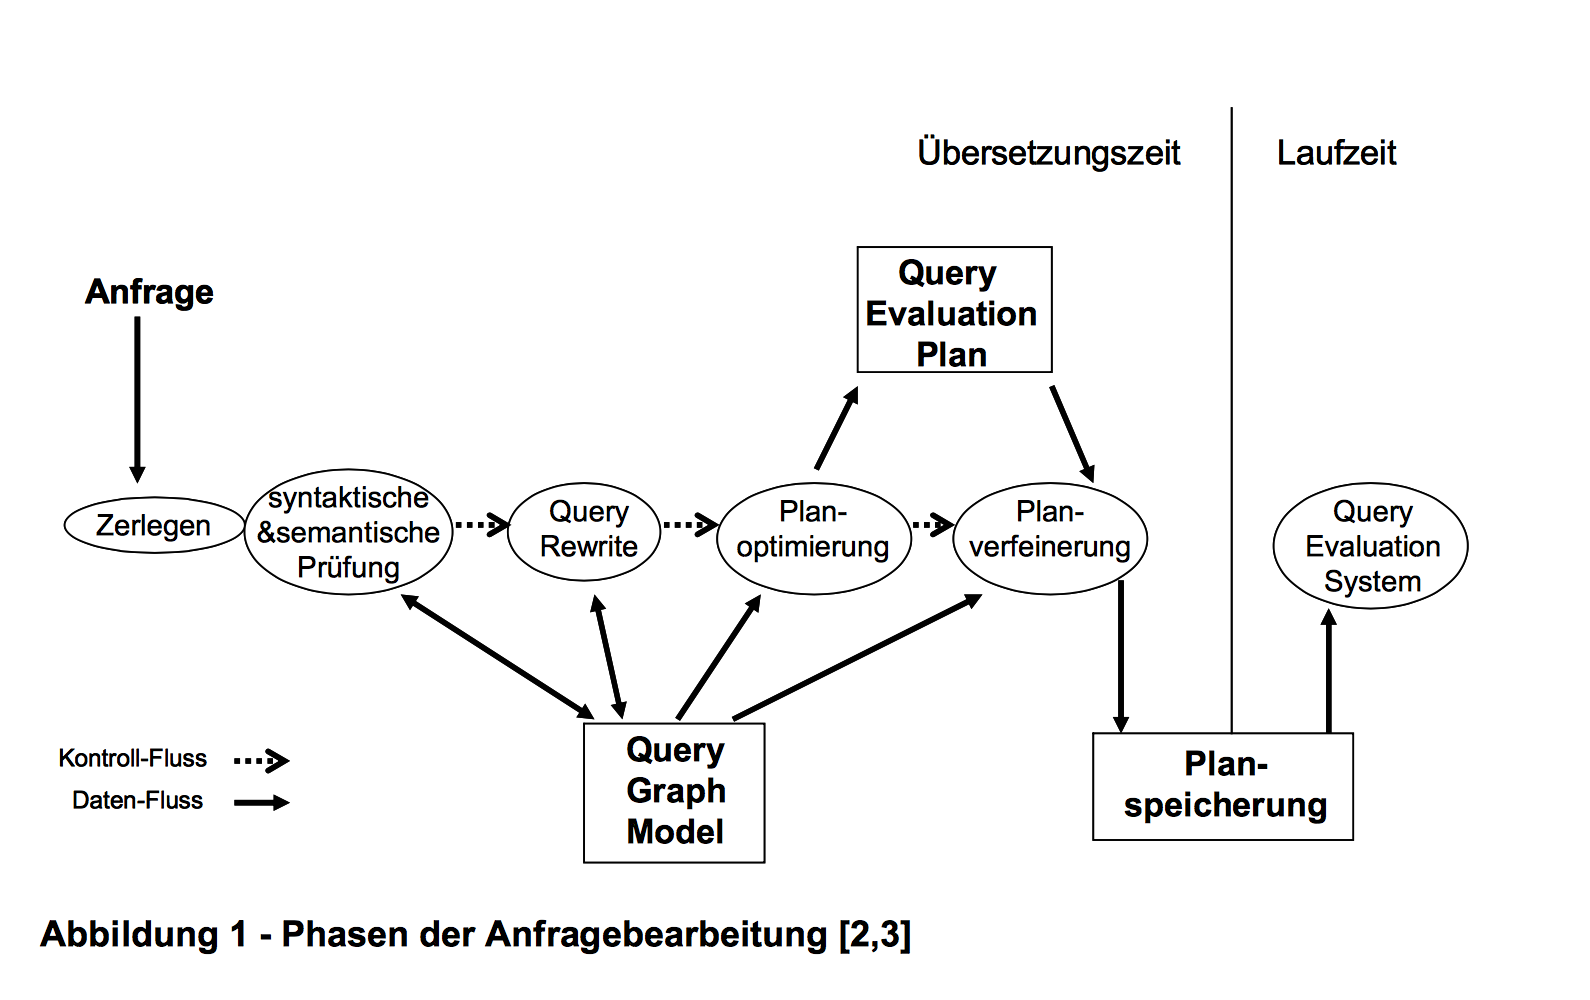
\includegraphics[width=\textwidth]{02_Grundlagen/Starburst.png}
  \caption{Starburst}
\end{figure}

Zur Comile-Time wird eine gegebene Anfrage auf semantische Korrektheit geprüft und in ein Query Graph Model (QGM) übersetzt. Basierend auf diesem QGM wird die Optimierungen der Anfrage durch zuerst einen Query Rewriter, einen Plan Optimierer und einen Plan Refiner durchgeführt.

Der Query Rewriter hat zwei konkrete Aufgaben: Auf der einen Seite soll die Anfrage in eine möglichst deklarative Form umgewandelt werden, hierbei werden insbesondere Anfragen entschachtelt. Auf der anderen Seite sollen weithin in der Forschung akzeptierte Heuristiken, beispielweise der Push-Down von Argumenten, angewandt werden.
Bei der Planoptimierung durchläuft der Plan vom QGM hin zu einem QEM drei Stationen. Die drei wesentlichen Aspekte sind der Plan Generator, die Berechnung der Plankosten und die Suchstrategie. 

\subsection{Regel-Maschine}

Zur Ausführung von Optimierungen wurde für die Starburst Datenbank eine eigene Regel-Maschine entwickelt \cite{lohman1988Starbust}. Diese Regelmaschine ist für die Anführung von Regelsets verantwortlich, die bei der Transformation der QGMs zur Anwendung kommen und durch den DBI  erweitert werden können. Die Regelmaschine basiert auf fünf Prinzipien:

\begin{enumerate}
\item Regel der arbiträren Komplexität: Eine Regel ist bei Starburst in zwei Teile aufgeteilt: Eine Koordinierungs- und eine Ausführungsfunktion. Bei dem Aufruf einer Regel muss zuerst geprüft werden, in wie weit die Regel angewendet werden darf. Ist sie anwendbar, wird die Ausführungsfunktion exekutiert.

\item Bei der Nutzung eines GQMs kann entweder eine Tiefen- als auch eine Breitensuche zur Anwendung kommen. Diese Art der Suche ist weder an die Regel noch an das Regel-Set geknüpft, sondern mit dem QGM selbst verbunden.


\item Die Regeln werden bei Starburst in Regelsets unterteilt. Ein Regel-Set besteht aus mehreren Regeln, die entweder sequenziell, nach einer vorab vergebenen Priorität oder einem statistischen Verfahren aufgerufen werden. Jede Regel und jedes Regel-Set kann andere Regeln und Regel-Sets als Teil einer Subroutine ausführen. _Neben der Funktion der Zusammenfassung der Regeln ist es Aufgabe der Regel-Sets._

\item Um die Ausführung von Transformationen zu limitieren, insbesondere bei der Ausführung des Rewriters, kann ein Budget vorgeschrieben werden. Sobald dieses Zeitbudget aufgebraucht ist, wird die Ausführung von Transformationsregeln abgebrochen. Es ist für diese Funktion unbedingt notwendig, dass Regeln immer vollständige QGMs zurückliefern, da sonst ein unvollständiger QGM als Resultat des Optimierers entstehen kann.

\item Schlussendlich ist es dem Nutzer der Datenbank möglich zu jedem beliebigen Zeitpunkt Regeln ausser Kraft zu setzen. Dies geschieht nur für den Nutzer lokal und andere Nutzer der Datenbank sind nicht betroffen. Spezielle Anwendungsfälle können so eine passgenau optimiert werden.
\end{enumerate}

\subsection{Plan Optimierer}

Der Plan Optimierer generiert basierend auf einem QGM mehrere alternative Query Evaluation Plans (QEPs). Für jeden dieser QEPs werden die Kosten geschätzt und der günstigste für die Weiterverarbeitung ausgewählt. Um die Erweiterbarkeit des Optimierers zu gewährleisten wurden die drei Komponenten (Plangenerierung, Kostenschätzung und Suchstrategie) von einander soweit getrennt, dass sie einzeln erweitert und verändert werden können. 

\subsection{Starburst Plan Generator}
$$HIER ÜBERARBEITEN$$
Der Plangenerator des Starburst Projekts, der für die Generierung von Planalternativen verantwortlich ist, bedient sich eines "Build Block"-Ansatzes[Lohm88] und einem Regel-Set, das auf einer eigenen Grammatik basiert.  

Als Build Block werden low-level-Datenbankoperationen (wie Access, Join und Sort) zu high-level Operationen kombiniert. Diese können wiederverwendet werden. Dank des Konzepts der Build Blocks ist es möglich die Erstellung und Verarbeitung in zwei wesendlichen Aspekten zu vereinfachen:


\begin{enumerate}


\item Die Regeln sind leichter von einem DBI zu lesen und zu verstehen, da die Fülle an Information mit Hilfe von Build Blocks aggregiert wurde.

\item Das Ausführen von Regeln wird effizienter. Da nicht mehr ganze Graphen nach Pattern durchsucht werden müssen, sondern direkt über Build Blocks erkannt werden, erleichtert sich die Ausführung. Ebenfalls ist es dank der Nutzung von Macro-Expandern möglich, die Geschwindigkeit zu verbessern.


\end{enumerate}


$$TEXT$$
Jede Regel erlabt es, dass aus ihr sowohl eine als auch mehrere Graphen entstehen können. In diesem Falle spricht man von Sets von Alternativen Plänen (SAP). 


\begin{itemize}
\item LOLEPOP
\item STARs
\end{itemize}

 